
\chapter{Simulation and Analysis tools}\label{mu2eana}

The Mu2e software framework has been designed to 
evaluate in advance the performance of the 
Mu2e detectors, assess signal reconstruction 
efficiency, and analyze the characteristics of 
background signals. This framework is built upon 
GEANT4, a widely recognized simulation toolkit 
that uses Monte Carlo methods for precise modeling.

Implemented in the C++ programming language, 
the framework encompasses a comprehensive suite of 
tools, including those for tracking, geometry 
configuration, and physics modeling. It provides 
detailed models of numerous physical processes, 
such as particle scattering, energy loss, and the 
decay of long-lived particles across a broad energy 
spectrum. The simulation environment faithfully 
reproduces the Mu2e geometry, and it integrates 
advanced pattern recognition and track reconstruction 
algorithms to enhance the accuracy and reliability of 
the simulations.

\section{art and FHiCL}

The Mu2e Offline software is structured around the \textit{art} framework 
(Figure \ref{fig:multistage}), a versatile system developed and maintained 
by the Fermilab Scientific Computing Division (SCD). This framework is 
utilized by several Intensity Frontier experiments at Fermilab due to its robustness and adaptability.

\textit{art} is an event-processing framework that is driven by command-line 
inputs and written in C++. It functions in a non-interactive mode, sequencing 
events as specified by the user. The framework is designed to address the 
extensive needs of high-energy physics experiments, including tasks such as 
high-level software triggering, online data monitoring, calibration, event 
reconstruction, simulation, and data analysis.

The configuration of \textit{art} at runtime is managed using the Fermilab 
Hierarchical Configuration Language (FHiCL), a specialized data definition 
language created at Fermilab. FHiCL files define the C++ classes that 
implement \textit{art} services. Within these classes, various algorithms -
ranging from simulation and reconstruction to analysis codes - are developed 
and compiled into dynamic libraries known as modules. The FHiCL files specify 
which modules will be loaded, the order in which they will be executed, and 
the input and output files involved in the process.

The simulation process is initiated using a FHiCL file, which configures 
the entire process by specifying the required modules and referencing 
additional files containing essential geometry and physics data.

\section{STNTUPLE and ROOT}

STNTUPLE is a data format for n-tuples and a lightweight n-tuple analysis 
framework written primarily in C++. Originally developed for the CDF 
experiment at Fermilab, it has been adapted for use in the Mu2e experiment. 
One of the \textit{art} plug-in modules is specifically designed for working 
with STNTUPLE \cite{stntuple}. Each STNTUPLE file is a ROOT file, which 
includes multiple branches corresponding to distinct data blocks. These 
blocks serve as optimized containers for I/O operations and analysis, 
storing Mu2e raw and/or reconstructed data. 

Using the appropriate module within the \textit{art}-job configuration 
file (with the .fcl extension), a STNTUPLE file can be generated from the 
data stored in an \textit{art} file. The data type stored in this format 
is highly customizable. Once the .stn file is produced, analysis can 
proceed directly from this data format, thereby eliminating the need 
to rerun the reconstruction process. STNTUPLE is built on the ROOT package, 
a data analysis and graphics software developed at CERN, enabling users to 
leverage all of ROOT's interactive features for their analysis.


\begin{figure}[!h]
    \centering
    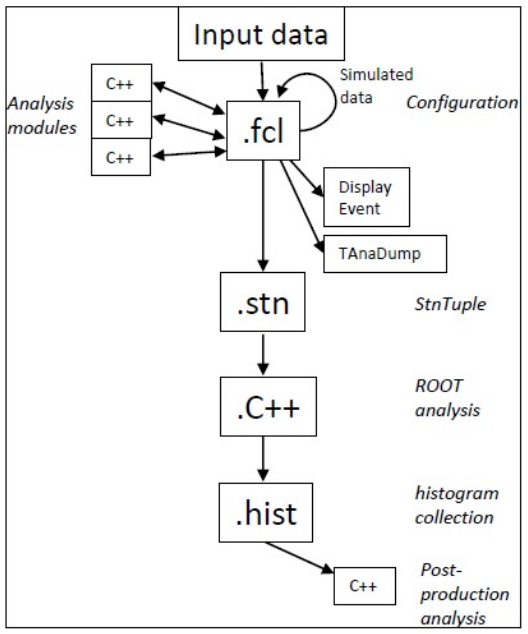
\includegraphics[width =0.4\textwidth]{figures/png/Screenshot_20240809_174458.png}
    \caption[Mu2e simulation and data handling.]{Both the generation and reconstruction 
    of events are performed through art-jobs configured using FHiCLs, which import the 
    necessary C++ modules. Additionally, modules such as the Event Display and TAnaDump 
    are utilized for debugging purposes. The analysis workflow relies heavily on the use 
    of STNTUPLE.
    }
    \label{fig:multistage}
\end{figure}

